% V3 v3_r04; working research draft, evidence-linked, human review required.
\documentclass[conference]{IEEEtran}
\usepackage[T1]{fontenc}
\usepackage{amsmath,amssymb,booktabs,url,tikz,pgfplots}
\pgfplotsset{compat=1.18}
\title{Endpoint Drift and Evaluation Sensitivity in Causal Visual Place Recognition: A Reproducible Study}
\author{\IEEEauthorblockN{Mingyang Zhou}\IEEEauthorblockA{University of Chinese Academy of Sciences\\\textit{Additional authors and correspondence pending}}}
\begin{document}\maketitle
\begin{abstract}
Sequence matching can improve visual place recognition while displacing its selected reference endpoint under a strict geographic matching threshold. We examine whether current-frame visual evidence can refine a coarse causal sequence prediction without adding an encoder. On already seen St Lucia data, a radius-four reference neighborhood covers 369 of 372 errors made by a fixed nine-image trajectory at a 10 m threshold. This is a diagnostic upper bound, not algorithm recall. We execute a bounded comparison of fixed temporal, encoder-fusion, naive local and score-support-constrained policies. On 656 seen validation queries, the selected constrained candidate retrieves 598 correctly at 10 m; the strongest non-candidate control retrieves 644. All configurations and unfavorable results are retained. Actual batch-one image pipelines have mean latencies 11.02 ms for CosPlace and 14.67 ms for the constrained candidate on the audited laptop GPU. New geographic validation could not be completed through the audited public sources, so the evidence does not establish an independently supported method contribution. The study separates candidate availability, baseline strength, label sensitivity and actual image-pipeline cost.
\end{abstract}
\begin{IEEEkeywords}visual place recognition, causal sequence matching, endpoint refinement, baseline comparison, reproducibility\end{IEEEkeywords}

\section{Introduction}
Visual place recognition (VPR) retrieves a reference image depicting a previously visited place~\cite{tutorial}. A global image descriptor provides an economical ranking, but appearance ambiguity can leave the best single-image match incorrect. A sequence of past observations can support a coherent reference trajectory. This motivates temporal matching, provided that past evidence does not erase current-frame discrimination between nearby places.

The evaluation protocol determines what constitutes a successful endpoint. A prediction can identify the correct route vicinity yet fail a tighter geographic threshold. Reference-index velocity also depends on image sampling, rather than physical speed. These distinctions become important when a long sequence selected on an ordinally aligned railway transfers to an irregularly sampled urban reference route with loops and geographic labels.

Our earlier frozen experiments found that a nine-image fixed trajectory performs strongly on Nordland, but short-window controls outperform it under strict St Lucia labels. These observations are already known: this study treats both datasets as seen development data. It does not rebrand the previous external test as independent because a new paper or new split is used.

We ask whether a coarse temporal endpoint usually has a valid neighboring reference, whether a simple current-frame reorder already extracts that opportunity, and whether an explicit temporal-support constraint adds value beyond strong fixed choices. We predeclare finite grids, common masks and a continuation rule before the new development outputs. The contribution offered here is an empirical mechanism and protocol audit. Sequence reasoning, local reranking and confidence-based trust are established; we claim neither their invention nor a new representation network.

\section{Related Work}
CosPlace~\cite{cosplace}, EigenPlaces~\cite{eigenplaces} and DINOv2~\cite{dinov2} supply frozen descriptors in our compact configurations. Their original best benchmark settings are not reproduced by this low-resolution experiment. The UPINLBS ResNet--Sinkhorn work~\cite{sameconference} addresses indoor global descriptors; only its publisher metadata was accessible, restricting detailed novelty comparison.

SeqSLAM~\cite{seqslam} and OpenSeqSLAM2.0~\cite{openseq} establish sequence trajectory reasoning and speed hypotheses. Our past-and-current cosine average is a disclosed descriptor-score adaptation, rather than an official reproduction of their grayscale normalization. Delta Descriptors~\cite{delta} transform temporal changes; their centered observation convention differs from our causal endpoint.

STA-VPR~\cite{sta} aligns CNN feature strips spatially and relaxes temporal alignment endpoints through local matching DTW. AdaptSeqVPR~\cite{adapt} describes variable sequence steps and a trained candidate discriminator in its publisher abstract; full text and official executable code were not verified. Thus, variable speed and flexible endpoints cannot be claimed as new ideas here. SMR~\cite{smr} learns when sequence matching helps or harms; its preserved earlier code adaptation is separate from the present untrained local-score candidate.

Local-image reranking~\cite{match} and similarity-distribution uncertainty~\cite{doubt} further constrain novelty. RRF~\cite{rrf} is a mature ranking fusion control. Our candidate's particular support inequality is tested against naive local visual and fixed local/global blending. A new combination of established operations, or improvement over an unfavorable long-window baseline, is insufficient evidence of a method contribution.

\section{Causal Endpoint Policies}
For image $I$, frozen encoder $f$ outputs unit descriptor $z(I)$. Current cosine scores are $S_t(j)=z(q_t)^\top z(d_j)$. A single-frame rank sorts $S_t$ stably in canonical gallery order. The causal coarse score is
\begin{equation}
T_t(j)=\max_{v\in\mathcal V}\frac{1}{L}\sum_{\ell=0}^{L-1} S_{t-\ell}\big(j-\operatorname{rint}(v\ell)\big).
\end{equation}
Only current and past query scores are used; $\operatorname{rint}$ rounds ties to even. Invalid or traversal-crossing reference paths have score $-\infty$. History resets at each split and query traversal. Before a complete window, the current visual rank is used.

Stable Top-$H$ distinct valid endpoints define $\mathcal C_t(H,r)$, the union of their bounded same-traversal reference-index neighborhoods, without nonmaximum suppression. Overlapping indices are deduplicated. We consistently remove indices with nonfinite $T_t$ from all local policies. This boundary convention is explicit: even an arbitrarily large support tolerance cannot restore a reference excluded by an invalid path. The radius counts reference images, not metres. Empty candidates or startup fall back to the visual ranking.

R0 sorts $T_t$. R1 sorts current $S_t$ inside $\mathcal C_t$; R3 is its $H=1$ alias. R2 sorts $(1-\gamma)(S_t+1)/2+\gamma(T_t+1)/2$ inside the same pool. The candidate P constrains admissibility:
\begin{equation}
\mathcal A_t=\{j\in\mathcal C_t:T_t(j)\ge \max_k T_t(k)-\varepsilon\}.
\end{equation}
It ranks $\mathcal A_t$ by current $S_t$, then appends every remaining reference in original visual order. R1/R2 use the same completion convention. All methods produce a full permutation with no duplicate or missing reference. At $\varepsilon=0$, maximum-$T$ ties are resolved by $S$; once $\varepsilon$ exceeds all finite candidate gaps, P equals R1. Neither $\gamma$ nor $\varepsilon$ is a probability or physical distance.

\begin{figure}[t]\centering
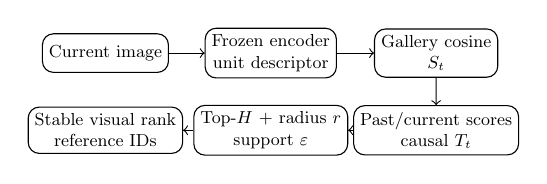
\begin{tikzpicture}[scale=.70,transform shape,every node/.style={draw,rounded corners,align=center,font=\small,minimum height=.7cm}]
\node (im) at (0,0) {Current image};\node (enc) at (3,0) {Frozen encoder\\unit descriptor};\node (sim) at (6,0) {Gallery cosine\\$S_t$};
\node (hist) at (6,-1.4) {Past/current scores\\causal $T_t$};\node (pool) at (3,-1.4) {Top-$H$ + radius $r$\\support $\varepsilon$};\node (rank) at (0,-1.4) {Stable visual rank\\reference IDs};
\draw[->] (im)--(enc);\draw[->] (enc)--(sim);\draw[->] (sim)--(hist);\draw[->] (hist)--(pool);\draw[->] (pool)--(rank);
\end{tikzpicture}
\caption{Image input to reference ranking. Query coordinates, labels and future images are absent. Geographic truth is used only after predictions for evaluation.}\label{fig:pipeline}
\end{figure}

\section{Protocol and Reproducibility}
\subsection{Seen Data and Ground Truth}
Nordland-Part-2020~\cite{nordland} provides 1750 summer references and aligned winter queries. Original training ordinals 1--600 and validation 701--1000 remain seen; main positives are within five reference ordinals. This is an index convention, not geographic distance. All validation methods exclude the first eight queries after history reset, giving 292 common queries.

St Lucia~\cite{stlucia}, in the source-pinned formatted benchmark~\cite{benchmark}, contains 1549 references and 1464 ordered queries. Its earlier results are already seen. V3 uses zero-based queries [0,700) for development, a [700,800) buffer unused for parameter selection, and [800,1464) for validation; common denominators are 692 and 656 after independent split resets. Whole-stream diagnostic comparisons have 1456 common queries. This conditional development selection is not a prospective blind test.

Euclidean UTM label distance defines 10 m primary and 25 m auxiliary positives; 5/15/50 m are declared sensitivities. At each radius every method shares the same no-positive exclusion and startup mask; no-positive counts and full-stream behavior are retained. Radius-dependent exclusions must be considered when comparing thresholds. Coordinates enter offline evaluation only. Reprojection of rounded St Lucia labels differs by up to 1.48305 m; a $\pm2$ m threshold band is recorded. This reprojection check establishes rounding consistency, not a bound on physical GPS sensor error, which is not surveyed here. Retrieval success is not estimated pose error or a 6DoF RMSE.

Reference-coordinate spacing is irregular: adjacent-gallery median 11.42 m and maximum 17.70 m, with source-frame gaps up to 345. Geographic route revisits can make distant reference indices correspond to nearby positions. The endpoint-to-visual index difference is therefore diagnostic only, not a metric localization error. All cache loads verify image-ID alignment, array hashes, model/checkpoint/source/preprocessing identities and manifest hashes. Required historical St Lucia Top10 predictions and Nordland key counts reproduce exactly. An independent scalar trajectory calculation, stable ranking check and CSV reaggregation check correctness; no-positive/startup behavior is recorded without method-dependent exclusions.

\subsection{Finite Search and Strong Controls}
All models use RGB ImageNet normalization and a bilinear antialiased 224-square tensor warp. CosPlace ResNet18/512, EigenPlaces ResNet50/512 and DINOv2 ViT-S14 CLS/384 are existing source/checkpoint-fingerprinted frozen encoders. No encoder or new classifier is trained.

Required temporal controls include $L9,v=1.2$ and full $\mathcal V=\{.8,1,1.2\}$ at $L=3,5,9$, alongside current-frame/global fixed blending, three A+B weights, RRF and shuffled past-score histories and reversed reference motion. With ties-to-even rounding, all three $L3$ velocity hypotheses yield offsets $[0,1,2]$; their identical paths preclude attributing an $L3$ gain to distinct speed adaptation.

The declared local grid is $H\in\{1,3\},r\in\{1,2,4,8\}$, $\gamma\in\{0,.25,.5,.75,1\}$ and $\varepsilon\in\{0,.01,.03,.06\}$. R1/R2 use all four temporal backends, totaling 32 and 160 configurations. P has 32 configurations on the original L9 backbone; this budget restriction precedes outputs. Selection is lexicographic seen-validation 10 m, then 25 m, then Nordland validation, then deterministic smaller parameters. P must exceed the strongest reasonable non-P control by at least two strict correct queries without auxiliary loss or more than one Nordland loss versus fixed L9. This is a continuation rule, not a significance test. No further module is added after candidate failure.

\subsection{Actual Image-Pipeline Measurement}
The frozen comparisons run on an RTX 3060 Laptop GPU using PyTorch 2.6.0/CUDA 12.4. Each receives 20 warm images and three complete 1464-image traversals at batch one, with CUDA synchronization and CPU/BLAS threads fixed to one. Every timed query reopens/decodes the image, prepares its tensor, runs the required encoder, transfers its descriptor, computes similarity, updates causal history and sorts the full gallery. Accuracy caches are used only for checks outside the timed interval. Model loading and a fresh batch 16 gallery build are measured separately. Measurements include this implementation's audit metadata, rather than a theoretical minimum matcher cost. The first real pass supplies the reported whole-stream prediction ledger; repeat and cache-score discrepancies are retained. RSS includes audit arrays and is separate from CUDA allocated/reserved memory. File cache is warm and GPU clocks are not locked; millisecond differences are descriptive, not deployment guarantees.

\section{Results and Mechanism Audit}
\subsection{Candidate Availability versus Algorithm Value}
On 1456 seen St Lucia diagnostic queries at 10 m, fixed L9 has 372 errors. Its $H1,r4$ neighborhood covers 369 of these; equal-size seed-zero uniform reference candidates cover six. The oracle fraction 99.19\% describes available positives, not a realizable policy. Of the paired A/T outcomes, 347 visual successes become temporal errors and 47 visual errors are rescued. The 25 m comparison changes to 20 harms and 34 rescues. These observations require matched thresholds and do not prove geometric localization accuracy.

The selected P uses $H=3,r=1,\varepsilon=0.06$ and retrieves 598/656 strict validation queries; the strongest non-P control retrieves 644/656. Its net difference is -46 correct queries. The declared development continuation gate is not met. This does not establish novelty or external generalization. Table~\ref{tab:main} uses the declared seen-validation splits. A strong short-window or local-blend control must be compared before interpreting an improvement over the original L9. All configuration-level and per-query evidence, including unsuccessful candidates, remains available.

\begin{table*}[!t]\centering\small
\caption{Already seen development validation, not independent testing. St Lucia has 656 queries at 10/25 m; Nordland has 292 at ordinal tolerance five. R1/R2/P use deterministic development-selected settings; percentages are derived from correct counts. Real seen-stream timing includes startup, measured as mean/median/P95 ms over 4392 queries per method.}\label{tab:main}
\begin{tabular}{lrrrrrrr}\toprule
Method & SL10 correct & SL10 \% & SL25 \% & Nordland \%  & Mean ms & Median ms & P95 ms\\\midrule
CosPlace A & 621 & 94.66 & 97.71 & 71.92 & 11.02 & 11.02 & 11.33\\
EigenPlaces B & 635 & 96.80 & 99.24 & 84.59 & 14.04 & 14.06 & 14.28\\
DINOv2 & 229 & 34.91 & 42.07 & 52.05 & 14.30 & 14.27 & 14.72\\
RRF & 630 & 96.04 & 99.09 & 83.22 & 23.62 & 23.61 & 23.92\\
A+B, B weight .75 & 639 & 97.41 & 99.70 & 85.62 & 23.37 & 23.38 & 23.60\\
Fixed L9, v1.2 & 495 & 75.46 & 98.93 & 99.66 & 12.14 & 12.13 & 12.36\\
Full-velocity L3 & 641 & 97.71 & 100.00 & 84.59 & 12.10 & 12.10 & 12.28\\
Full-velocity L5 & 638 & 97.26 & 100.00 & 89.73 & 12.38 & 12.37 & 12.59\\
Full-velocity L9 & 626 & 95.43 & 99.85 & 97.26 & 13.19 & 13.28 & 13.55\\
Global L9 blend .75 & 593 & 90.40 & 99.70 & 98.97 & 12.29 & 12.29 & 12.49\\
Local visual R1 & 636 & 96.95 & 100.00 & 84.59 & 15.17 & 15.17 & 15.35\\
Local fixed blend R2 & 644 & 98.17 & 100.00 & 82.53 & 14.93 & 14.93 & 15.14\\
Support candidate P & 598 & 91.16 & 99.54 & 97.60 & 14.67 & 14.67 & 14.86\\
\bottomrule\end{tabular}\end{table*}

\begin{table}[!t]\centering\small
\caption{Prescribed support/local ablations on seen St Lucia validation (656 common queries). Every value refers to a complete frozen ranking. Full 224-configuration grid is archived.}\label{tab:ablation}
\begin{tabular}{lrr}\toprule
Policy & 10m correct & 25m correct\\\midrule
$H1,r1,\varepsilon0$ & 495 & 649\\
$H1,r1,\varepsilon0.01$ & 502 & 648\\
$H1,r1,\varepsilon0.03$ & 526 & 649\\
$H1,r1,\varepsilon0.06$ & 564 & 651\\
$H3,r8,\varepsilon.06$ & 598 & 653\\
P pool, no support & 631 & 655\\
P pool, fixed blend .5 & 630 & 655\\
P pool, fixed blend 1 & 495 & 649\\
\bottomrule\end{tabular}\end{table}

\begin{figure}[t]\centering
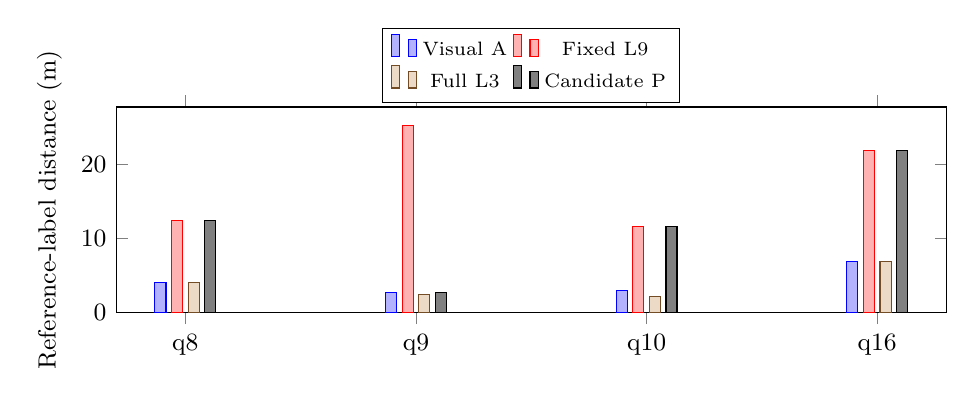
\begin{tikzpicture}\begin{axis}[width=\columnwidth,height=1.65in,ybar,bar width=4pt,symbolic x coords={q8,q9,q10,q16},xtick=data,ymin=0,ylabel={Reference-label distance (m)},legend style={at={(.5,1.02)},anchor=south,font=\scriptsize,legend columns=2},tick label style={font=\small},label style={font=\small}]
\addplot coordinates {(q8,4.053949) (q9,2.708357) (q10,2.999233) (q16,6.851839)};\addlegendentry{Visual A}
\addplot coordinates {(q8,12.372752) (q9,25.213316) (q10,11.580799) (q16,21.803128)};\addlegendentry{Fixed L9}
\addplot coordinates {(q8,4.053949) (q9,2.421611) (q10,2.178302) (q16,6.851839)};\addlegendentry{Full L3}
\addplot coordinates {(q8,12.372752) (q9,2.708357) (q10,11.580799) (q16,21.803128)};\addlegendentry{Candidate P}\end{axis}\end{tikzpicture}
\caption{Real seen cases in traversal order: q8/q16 have repairable neighborhoods; q9/q10 have no positive in the H1/r16 finite-T pool. Labels are geographic retrieval distances, not estimated poses. Photos and full IDs remain local in the case evidence.}\label{fig:cases}\end{figure}

\subsection{Cases, Sensitivity and Boundary Failure}
Eight real cases follow the declared first-two-in-traversal-order rule for repairable drift, unavailable H1-neighborhood truth, visual success harmed by sequence matching, and multiwindow disagreement. Query 16 illustrates nearby endpoint drift: visual/L3 reference distance is 6.9 m versus 21.8 m for fixed L9. Queries 9 and 10 expose the finite-path boundary: valid sequence indices can exclude early nearby references, while other loops provide competing reference identities. A reference-index difference is therefore not geographic error, especially with route revisits.

The initial case audit used H3 for its unavailable-neighborhood category, found no matching query, and explicitly flagged fallback examples. A preserved supplement applies the specified Top1-centered H1 condition and verifies the named categories. This correction affects interpretation, not scores, parameters or prediction selection. Photographs are available locally through their image IDs/rebuild script; uncertain redistribution rights prevent including them in this public draft. Numeric case panels preserve the actual failure evidence.

All prescribed tolerances, distance medians/P90/P95, near-boundary counts, rescues/harms and contiguous 100-query blocks are retained. Blocks are descriptive because adjacent video frames are correlated; neither query count nor three timing repeats is treated as independent trials. The exact winning coarse velocity/path offsets are recorded in the frozen real-image ledger; earlier development ledgers' \texttt{path\_offsets} denote the first hypothesis and are not claimed to be winning paths. The archival audit preserves failed test collection, public-source access and oversized-ZIP checkpoint records. The first complete ZIP was kept unchanged and divided into sub100MB byte chunks; subsequent lossless ZIPs have indexed parts and checksums. No negative configuration, difficult query, old manuscript or freeze was overwritten. The corresponding human review checklist marks independent generalization, partial source access, photo rights and final conference requirements unresolved.

\section{Discussion and Conclusion}
A broad candidate oracle establishes that local reference availability is often sufficient; it does not establish that temporal support filtering beats current-frame ranking or a short fixed window. Our bounded implementation tests that distinction against mature controls, with complete causal rankings and exact query ledgers. The strongest fixed or simple local method, rather than a weak historical method, sets the incremental contribution bar.

All accuracy evidence is development or descriptive seen-data evidence. Oxford RobotCar's official RTK source~\cite{robotcar} is promising, but camera downloads require registration. The SFU Mountain source~\cite{sfu} supplies licensed ordered images and manual place correspondences; necessary official archives failed normal public HTTP/HTTPS access in our bounded audit. SFU's approximate annotation spacing and GPS accuracy would not validate strict 10 m geographic improvement even if those bundles became available. No new independent image performance is reported, and no alternative is selected using model scores.

Consequently, this is a working empirical draft, not an independently validated new-method submission. Correlated video frames, rounded geographic labels, reference loops, one limited P backbone grid, unavailable external data and partial related-paper access restrict the conclusion. Actual evidence and prior manuscripts are preserved for human review. Further external validation would require a fresh metadata audit and prospective freeze, rather than retuning on an opened test.

\section*{Acknowledgment}
OpenAI ChatGPT/Codex assisted with the V3 implementation, experimental execution and analysis, figures, and drafting/editing of the abstract and Sections I--VI. Human authors must review all claims, citations and AI-assisted content and remain responsible for the manuscript. Author list/order, correspondence, affiliation wording and funding require human confirmation; no submission or copyright action has been performed.

\clearpage
\begin{thebibliography}{20}
\bibitem{tutorial} S. Schubert, P. Neubert, S. Garg, M. Milford, and T. Fischer, ``Visual place recognition: A tutorial,'' \emph{IEEE Robot. Autom. Mag.}, vol.31, no.3, pp.139--153, 2024, doi:10.1109/MRA.2023.3310859.
\bibitem{cosplace} G. Berton, C. Masone, and B. Caputo, ``Rethinking visual geo-localization for large-scale applications,'' in \emph{CVPR}, 2022, pp.4878--4888.
\bibitem{eigenplaces} G. Berton, G. Trivigno, B. Caputo, and C. Masone, ``EigenPlaces: Training viewpoint robust models for visual place recognition,'' in \emph{ICCV}, 2023, pp.11080--11090.
\bibitem{dinov2} M. Oquab \emph{et al.}, ``DINOv2: Learning robust visual features without supervision,'' arXiv:2304.07193, 2023.
\bibitem{seqslam} M. J. Milford and G. F. Wyeth, ``SeqSLAM: Visual route-based navigation for sunny summer days and stormy winter nights,'' in \emph{ICRA}, 2012, pp.1643--1649, doi:10.1109/ICRA.2012.6224623.
\bibitem{openseq} B. Talbot, S. Garg, and M. Milford, ``OpenSeqSLAM2.0: An open source toolbox for visual place recognition under changing conditions,'' arXiv:1804.02156v2, 2018.
\bibitem{delta} S. Garg, B. Harwood, G. Anand, and M. Milford, ``Delta descriptors: Change-based place representation for robust visual localization,'' \emph{IEEE Robot. Autom. Lett.}, vol.5, no.4, pp.5120--5127, 2020, doi:10.1109/LRA.2020.3005627.
\bibitem{smr} S. Hussaini, T. Fischer, and M. Milford, ``Improving visual place recognition with sequence-matching receptiveness prediction,'' in \emph{IROS}, 2025, pp.11073--11080, doi:10.1109/IROS60139.2025.11247581.
\bibitem{match} D. Sferrazza, G. Berton, G. Trivigno, and C. Masone, ``To match or not to match: Revisiting image matching for reliable visual place recognition,'' in \emph{CVPR Workshops}, 2025, pp.2874--2885.
\bibitem{doubt} E. Miller, M. Milford, M. B. Hafez, S. Ramchurn, and S. Ehsan, ``Through the lens of doubt: Robust and efficient uncertainty estimation for visual place recognition,'' \emph{IEEE Robot. Autom. Lett.}, vol.11, no.5, pp.5899--5906, 2026, doi:10.1109/LRA.2026.3674688.
\bibitem{rrf} G. V. Cormack, C. L. A. Clarke, and S. B\"uttcher, ``Reciprocal rank fusion outperforms condorcet and individual rank learning methods,'' in \emph{SIGIR}, 2009, pp.758--759, doi:10.1145/1571941.1572114.
\bibitem{sameconference} Y. Wei, Y. Li, and Z. Zheng, ``Balancing accuracy and efficiency: A ResNet--Sinkhorn framework for extracting global image descriptors in indoor visual place recognition,'' in \emph{UPINLBS}, 2025, pp.1--6, doi:10.1109/UPINLBS68186.2025.11468446.
\bibitem{stlucia} M. J. Milford and G. F. Wyeth, ``Mapping a suburb with a single camera using a biologically inspired SLAM system,'' \emph{IEEE Trans. Robot.}, vol.24, no.5, pp.1038--1053, 2008, doi:10.1109/TRO.2008.2004520.
\bibitem{benchmark} G. Berton, R. Mereu, G. Trivigno, C. Masone, G. Csurka, T. Sattler, and B. Caputo, ``Deep visual geo-localization benchmark,'' in \emph{CVPR}, 2022, pp.5396--5407.
\bibitem{nordland} S. Garg, ``Nordland-Part-2020,'' Zenodo, 2020, doi:10.5281/zenodo.4016653.
\bibitem{sta} F. Lu, B. Chen, X.-D. Zhou, and D. Song, ``STA-VPR: Spatio-temporal alignment for visual place recognition,'' \emph{IEEE Robot. Autom. Lett.}, vol.6, no.3, pp.4297--4304, 2021, doi:10.1109/LRA.2021.3067623.
\bibitem{adapt} H. Li, G. Peng, J. Zhang, S. Vaikundam, and D. Wang, ``AdaptSeqVPR: An adaptive sequence-based visual place recognition pipeline,'' in \emph{IROS}, 2023, pp.3284--3289, doi:10.1109/IROS55552.2023.10341533.
\bibitem{robotcar} Oxford Robotics Institute, ``Oxford RobotCar Dataset: RTK ground truth,'' 2020. [Online]. Available: \url{https://robotcar-dataset.robots.ox.ac.uk/ground_truth/}
\bibitem{sfu} J. Bruce, J. Wawerla, and R. Vaughan, ``The SFU Mountain dataset: Semi-structured woodland trails under changing environmental conditions,'' in \emph{ICRA Workshop on Visual Place Recognition in Changing Environments}, 2015.

\end{thebibliography}
\end{document}
